\documentclass[tikz]{standalone}

\usepackage{amsmath}
\usepackage{physics}

\usetikzlibrary{arrows.meta,fit,positioning}

\begin{document}
	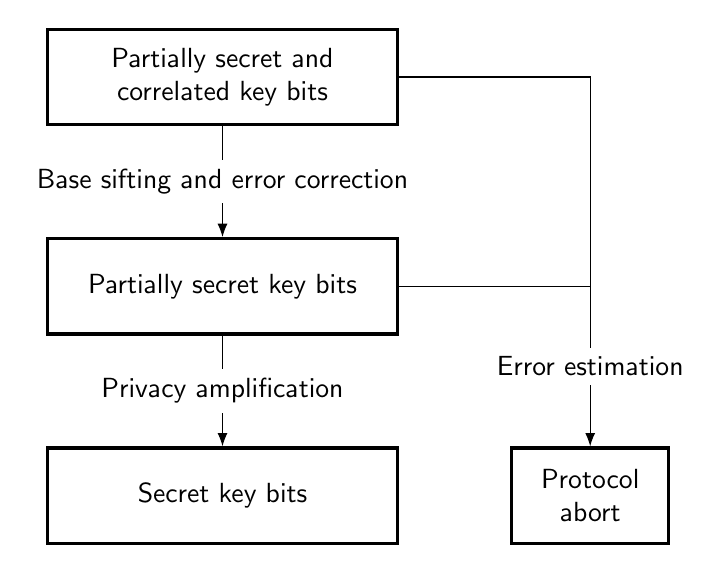
\begin{tikzpicture}[
		node distance=4em,
		block/.style={draw, very thick, minimum height=8ex, minimum width=3.5em, align=center, text width=12em},
	]
		\node (kb1) [block] {\textsf{Partially secret and correlated key bits}};
		\node (kb2) [block, below=of kb1] {\textsf{Partially secret key bits}};
		\node (kb3) [block, below=of kb2] {\textsf{Secret key bits}};
		
		\draw[-Latex] (kb1) -- (kb2) node[midway, fill=white] {\textsf{Base sifting and error correction}};
		\draw[-Latex] (kb2) -- (kb3) node[midway, fill=white] {\textsf{Privacy amplification}};
		
		\node (abort) [block, right=of kb3, text width=5em] {\textsf{Protocol abort}};
		\draw[-Latex] (kb2) -- (abort|-kb2) -- (abort) node[midway, fill=white] {\textsf{Error estimation}};
		\draw (kb1) -- (abort|-kb1) -- (abort|-kb2);
	\end{tikzpicture}
\end{document}